\chapter{Introduction}

Almost everyone uses the internet everyday, whether connecting to the internet from their mobile devices or browsing the internet on their personal computers. It is safe to say that most of us will struggle with everyday activities without devices that are capable to connect to the internet. For example, getting a taxi ride, ordering food delivery or even navigating to places we want to go. Apple have made an interesting short movie "predicting" what might happen without Apps on mobile devices during their annual Worldwide Developers Conference (WWDC) in 2017 [15].
 
Internet have an even greater presents and role within the science and engineering community, sites like Google Scholar and The New England Journal of Medicine have benefited scientists, doctors and engineers greatly [15] [16] [17]. Prior to the wide adaption of the internet, searchers, scholars and students would spend countless hours in physical libraries, browsing through hundreds of thousands of academic journals and books in order to answer one question or to solidify a proposal they had in mind. Today with the help of the internet, it will hardly take a few minutes. This leads to the jump in research productivity which helps researchers and engineers to produce their research and production output to a new level, thus allowing them to essentially do more things with the same amount of time.
 
For the last 20 years, PHP and JavaScript are the technologies that dominates the majority of web browsers and web development. Although updates and new versions are issued regularly, they are still becoming more aged everyday, and software engineers have been finding ways to improve the performance, user experience and developer experience for this ageing technology. For example, Microsoft developed the Typescript language to combat the "strange" nature of the JavaScript language [18], and to help resolving the lack of type checking within JavaScript [19]. Facebook developed the "React" library framework to improve developer experience by introducing the "component" concept. Where each class or function within a React project can be seen as a UI (user interface) component. This can be a button, a table or a component with more complexity, such as a navigation header component [20]. As expected and intended, some of the popular web development frameworks and libraries such as React JS and Angular (Google) have gained significant attention and much of the industry-wide adaption since their release and they have indeed significantly improved browsing experience for all of us.
 
However, little did we know, a major change was just around the corner.
 
\bigskip
\bigskip

\textbf{{\Large Chapter 1.1 Meet WebAssembly}}

\bigskip

WebAssembly was first released and adopted in 2017 by a number of browsers [21]. Since then, there has been a growing community built around the technology as more and more projects started using WebAssembly. As mentioned above, JavaScript have been the de facto language for web browsers since the beginning of the web. However, this was never the original intention during the initial development of JavaScript.

There is a wide spread misconception that Al Gore, the Former Vice President of the United States, invented the internet. However, this is not true as Al Gore has never claimed or said so. Instead, what he actually said was "I took the \textbf{initiative} in creating the internet" during his interview with CNN in 1999 [22]. However, AL Gore did introduced the High Performance Computing Act of 1991 [23], which help funded the creation of the first mainstream web browser Mosaic [24], as well as the creation of the high-speed fiber optic computer network [25].

JavaScript was born not long after the release of the first version of Netscape Navigator - the most popular web browser in the late 90s. It was written by Brendan Eich and it only took him 10 days to release the first version [26]. Initially, JavaScript did not gain that much attention and it wasn't until the release of Internet Explorer version 3 which added the support for the language which then popularised it to the general public [27] [28]. Growing up alongside the internet, JavaScript have had quite a number of iterations and feature upgrades. Although it is indeed powerful and popular, in recent years, developers and engineers started to see JavaScript as a "messy" language [figure \ref{fig:javascript_meme}]. That is when developers and major tech companies came up with the idea of creating a brand new language based on all the experience and mistakes from the last 20 years. Therefore, in 2017, WebAssembly was introduced.

\newpage

\begin{figure}[hp]
\centering
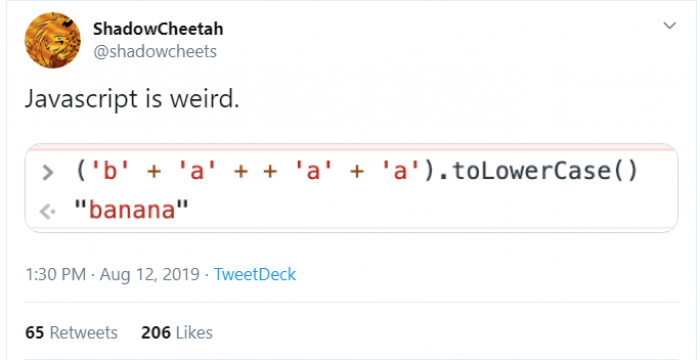
\includegraphics[scale=0.7]{javascript_meme}
\caption{\footnotesize{Internet "meme" about the JavaScript language.}}
\captionsetup{aboveskip=0pt,font=it}
\label{fig:javascript_meme}
\end{figure}

\bigskip

WebAssembly is the first widely adopted language that was built entire from the ground up with a formal semantics as well as to work in the area it originally intended to which is large, complex apps running on modern web browsers. WebAssembly have an incredibly clean and simple yet powerful design such as memory allocation and garbage collection [21]. However, WebAssembly is actually a form or binary code. Developers and engineers don't usually write WASM code directly, instead they write programs with other low-level languages such as c, c++ or rust [29].

\bigskip
\bigskip

\textbf{{\Large Chapter 1.2 Meet WebAssembly}}

\bigskip

Test